\graphicspath{{./figures}}

\section{Ground Station Antenna}

The ground station antenna's return loss was measured using a network analyser to ensure it was correctly matched to $\SI{50}{\ohm}$. The resultant graph is shown in Figure \ref{fig:helicalReturnLoss}. The figure shows that the simple matching strip design is effective and was implemented correctly, however it should be noted that the null is not as deep as simulated (only around -10 dB minimum at 427 MHz as opposed to the -35 dB simulated minimum at the centre frequency of 433 MHz). This may either be due to the aluminium foil used being far from an ideal PEC, or most likely due to the imperfections in the antenna's construction (e.g. bends in the coil, the added dielectric resonance due to the PVC and wooden dowels etc.). Instead of optimizing the antenna build, however, it was decided to run further tests with the system as-is, since the link budget allows for up to a 1 dB matching loss. Optimisation is therefore left for future projects. Lastly, the antenna pattern unfortunately could not be measured, as a chamber was not available that could measure the desired frequency range.


\begin{figure}[!tb]
  \begin{minipage}{.49\textwidth}
    \centering
    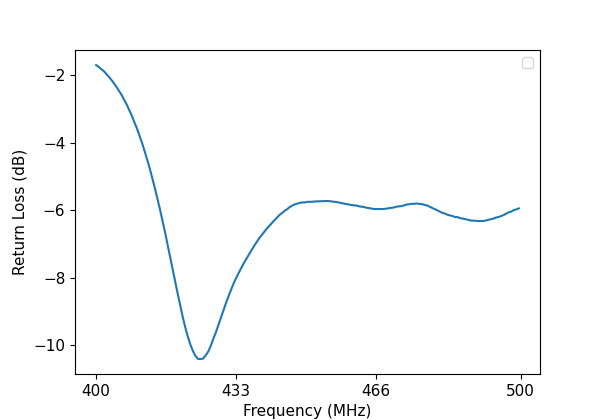
\includegraphics[width=1.0\linewidth]{helicalReturnLoss}
    \caption{Measured Helical Antenna Return Loss vs Frequency}
    \label{fig:helicalReturnLoss}
  \end{minipage}
  \begin{minipage}{.49\textwidth}
    \centering
    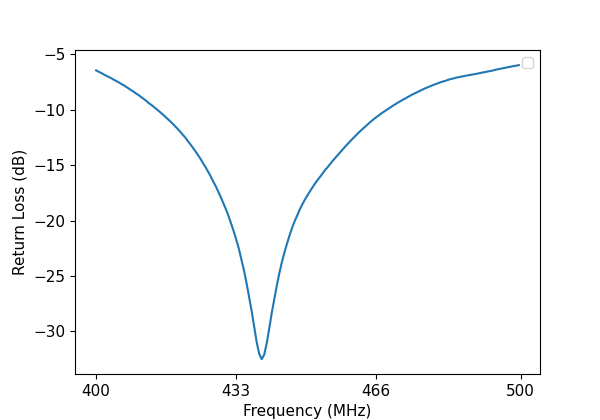
\includegraphics[width=1.0\linewidth]{dipoleReturnLoss}
    \caption{Measured Dipole Antenna Return Loss vs Frequency}
    \label{fig:dipoleReturnLoss}
  \end{minipage}
\end{figure}